% !TeX program = xelatex
% Self-contained Beamer deck: copy this file alone and run XeLaTeX twice.
% Uses standard TeX Live packages and fonts; no project assets or shell escape.
% Allow Computer Modern math at the exact requested sizes.
\RequirePackage{fix-cm}
\documentclass[10pt,aspectratio=169]{beamer}
\geometry{paperwidth=180mm,paperheight=101.25mm}
\usepackage{fontspec}
\setsansfont{texgyreheros}[Extension=.otf,UprightFont=*-regular,BoldFont=*-bold,ItalicFont=*-italic,BoldItalicFont=*-bolditalic]
\setmonofont[Scale=0.88,BoldFont=lmmonolt10-bold.otf,ItalicFont=lmmono10-italic.otf,BoldItalicFont=lmmonolt10-boldoblique.otf]{lmmono10-regular.otf}
\usepackage{booktabs,tabularx,array,tikz}
\usetikzlibrary{arrows.meta,positioning,calc,shapes.geometric}
\definecolor{Navy}{HTML}{17324D}
\definecolor{Teal}{HTML}{007F82}
\definecolor{Blue}{HTML}{4178B5}
\definecolor{Amber}{HTML}{A86B17}
\definecolor{Slate}{HTML}{586878}
\definecolor{Pale}{HTML}{F0F4F7}
\setbeamercolor{normal text}{fg=Navy,bg=white}
\setbeamercolor{structure}{fg=Teal}
\setbeamercolor{frametitle}{fg=Navy}
\setbeamerfont{frametitle}{size=\Large,series=\bfseries}
\setbeamercolor{block title}{fg=Navy,bg=Pale}
\setbeamercolor{block body}{fg=Navy,bg=Pale}
\setbeamerfont{block title}{size=\normalsize,series=\bfseries}
\setbeamertemplate{navigation symbols}{}
\setbeamersize{text margin left=7mm,text margin right=7mm}
\setbeamertemplate{headline}{\vspace{2mm}\hspace{7mm}{\color{Teal}\fontsize{7.5}{9}\selectfont\bfseries TRACE-Q\quad /\quad\insertsectionnumber\enspace\MakeUppercase{\insertsectionhead}}\vspace{1mm}}
\setbeamertemplate{frametitle}{\vspace{0mm}\insertframetitle\par\vspace{1mm}}
\setbeamertemplate{footline}{\hspace{7mm}{\color{Slate}\fontsize{6.8}{8}\selectfont FINAL HUMAN REVIEW v2.4.1\quad |\quad OCTOBER 22, 2026}\hfill{\color{Slate}\fontsize{7.5}{9}\selectfont\insertframenumber\,/\,\inserttotalframenumber}\hspace{7mm}\vspace{2mm}}
\setbeamertemplate{itemize item}{\color{Teal}\small\textbullet}
\setlength{\tabcolsep}{5pt}
\renewcommand{\arraystretch}{1.16}
\newcolumntype{Y}{>{\raggedright\arraybackslash}X}
\newcommand{\code}[1]{{\ttfamily\fontsize{8}{9.5}\selectfont\detokenize{#1}}}
\newcommand{\src}[1]{\par\vfill{\color{Slate}\fontsize{6.5}{8}\selectfont #1\par}}
\newcommand{\takeaway}[1]{\par\medskip{\color{Teal}\bfseries #1}\par}
\newcommand{\smalltext}{\fontsize{8.5}{10.4}\selectfont}
\hypersetup{pdftitle={TRACE-Q: Study Design, Review Notes and Before/After Publication-Cohort Comparisons},pdfauthor={},pdfsubject={Three-section presentation based on the October 22, 2026 manuscript and final v2.4.1 human review workbooks}}


\begin{document}

\section{Paper and study design}

\begin{frame}[t]{TRACE-Q: study design, review evidence and period changes}
\vspace{1mm}
{\large An exploratory toolkit for evidence-grounded review\\of quantitative research reporting}\par
\vspace{4mm}
\begin{columns}[T,onlytextwidth]
\column{.31\textwidth}
{\color{Blue}\fontsize{30}{32}\selectfont\bfseries 139}\par
\textbf{Confirmed all}\par
\small Statistical findings of any\newline substantive importance
\column{.31\textwidth}
{\color{Teal}\fontsize{30}{32}\selectfont\bfseries 37}\par
\textbf{Confirmed substantive}\par
\small Subset with potential to affect\newline interpretation or data use
\column{.31\textwidth}
{\color{Navy}\fontsize{30}{32}\selectfont\bfseries 44}\par
\textbf{Trial packages}\par
\small 19 earlier and 25 later reports\newline from selected JAMA trials
\end{columns}
\vspace{5mm}
\begin{tabularx}{\linewidth}{@{}rY@{}}
\textcolor{Teal}{\textbf{01}} & Study design: 44 trial packages and final human review.\\
\textcolor{Teal}{\textbf{02}} & Codebook and text mining: link raw notes to final human decisions.\\
\textcolor{Teal}{\textbf{03}} & Before/after cohorts: statistical findings and the other three domains.
\end{tabularx}
\src{Source: TRACE-Q draft and supplement, October 22, 2026; four completed human review workbooks. Here, ``confirmed all'' refers specifically to statistical findings with original report-only relationships.}
% BEGIN EMBEDDED SPEECH NOTE
% Final judgments: review_results_2_4_1_Rbulun_copy/*.xlsx.
\note{
汇报路线：研究设计、审查规则与时期变化
\par
今天的汇报以 review\_results\_2\_4\_1\_Rbulun\_copy 文件夹中四份 completed 工作簿的最终审查结果为依据。第一部分介绍 TRACE-Q 研究设计与论文样本；第二部分说明 codebook 如何把候选条目转化为可汇总的判断；第三部分比较早期与后期发表队列。原始说明的机制分类作为补充分析单独介绍。
\par
我们重新读取了四份工作簿的候选工作表，逐项核对处置、最终领域、完成状态、证据判断和实质性。统计结果中，已确认的问题共 139 个，其中 37 个具有实质性。37 是 139 的子集，不能相加。下面的数量和时期比较都以这些最终判断为准。
\par
这里的疫情前后，具体指 2018 至 2019 年和 2024 至 2025 年发表的论文，不是按每个试验的招募时间分组，也不是疫情影响的因果研究。文本分析也有明确边界：只重新分类 statistical\_results 中已确认的问题。其他三个领域仅用于单独的时期比较。
\par
转场：先介绍实际纳入的论文和审查资料。
}
% END EMBEDDED SPEECH NOTE
\end{frame}





\begin{frame}[t]{The comparison uses 44 selected trial packages}
\begin{columns}[T,onlytextwidth]
\column{.59\textwidth}
\small
\begin{tabular}{@{}lrrrr@{}}
\toprule
Year & Papers & PDF pages & Flags & Retained\\\midrule
2018 & 10 & 1,070 & 115 & 107\\
2019 & 9 & 994 & 79 & 76\\
2024 & 10 & 1,097 & 113 & 107\\
2025 & 15 & 2,398 & 133 & 123\\\midrule
\textbf{Total} & \textbf{44} & \textbf{5,559} & \textbf{440} & \textbf{413}\\\bottomrule
\end{tabular}
\medskip\par
188 PDFs plus one supplementary Excel worksheet. Plans may be embedded in supplements.
\medskip\par
\textbf{Period denominators}\par
2018--2019: \textbf{19 papers}\quad 2024--2025: \textbf{25 papers}
\column{.36\textwidth}
\begin{block}{Human review}
\small
413 retained; 27 excluded.\\
All 440 entries completed; no deferred dispositions.\\[2mm]
Final copied workbooks were later human-reviewed (user-confirmed). Raw \code{R_Bulun} notes came from earlier AI review runs.
\end{block}
\small
Availability sample of primary randomized JAMA trials in the selected publication years. No complete journal screening log.
\end{columns}
\takeaway{Before = 2018--2019; after = 2024--2025 publication cohorts.}
\src{Source: manuscript, Application and Results; analysis/year\_summary.csv. Cohort follows recorded online-first year, which can differ from the DOI year. Raw notes are AI-authored; final labels are human-reviewed. Period labels do not identify a pandemic effect.}
% BEGIN EMBEDDED SPEECH NOTE
% Final judgments: review_results_2_4_1_Rbulun_copy/*.xlsx.
\note{
样本：44 个试验资料包与最终人工处置
\par
四份最终工作簿对应 44 篇论文：2018 年 10 篇，2019 年 9 篇，2024 年 10 篇，2025 年 15 篇。早期是 19 篇，后期是 25 篇。年份按工作簿的候选编号和 Papers 清单确定，不能只根据 DOI 中的年份分组。
\par
逐年候选数是 115、79、113 和 133；保留数是 107、76、107 和 123。合起来有 440 个候选、413 个保留和 27 个排除。每个候选的完成状态都是 primary\_done，没有 discuss 处置。保留并不等于已确认统计错误，各领域还要按自己的判断字段继续筛选。
\par
这页的 188 个 PDF、5,559 页和补充 Excel 是原有资料清单描述的材料规模，并不是本次从审查工作簿重新计算的结果。核心分析的分母仍然是 44 篇论文，不能把每一页或每个候选当成独立的论文观察值。
\par
研究采用资料可获得性样本，不能代表期刊所有随机试验。工作簿提供最终判断，但现有资料没有可识别的独立人工双人评分，因此不能用这些结果估计评审者间一致性。
\par
还有一个影响讲稿解释的事实：最终工作簿中，413 条保留记录的 Notes 全部为空；非空说明只出现在 27 条排除记录中。因此，后面的确认数和实质性数可以直接核对，机制类别和具体解释则不能声称来自这些最终工作簿的说明栏。
\par
转场：接着用 codebook 说明，保留一个条目究竟代表什么。
}
% END EMBEDDED SPEECH NOTE
\end{frame}

\section{Review codebook and Notes mining}

\begin{frame}[t]{Common fields establish a traceable human decision}
\smalltext
\begin{tabularx}{\linewidth}{@{}p{2.9cm}Y@{}}
\toprule
Field (column) & Operational rule in codebook v2.4.1\\\midrule
Identity and evidence (A--C) & Preserve the candidate key; the title is a flag, not a verdict. Open the original file and PDF page named in the source location.\\
Review domain (E) & Choose the assessment branch first. The AI suggestion is editable; the original document relationship code stays frozen.\\
Disposition (D) & \code{retain}: keep for applicable summaries; \code{exclude}: remove after assessment; \code{discuss}: considered but deferred. A blank means unanswered.\\
Completion (F) & Use \code{no} while drafting and \code{primary_done} after manual review. Reset to \code{no} before editing a completed row; then review and complete again.\\
Validation hint (G) & Calculated \code{PRIMARY READY} means valid entry plus manual completion, including a deferred \code{discuss} decision. It does not certify scientific accuracy.\\
Notes (R) & Optional English context; no inherited answers. Clear obsolete literal answers when changing branches.\\\bottomrule
\end{tabularx}
\medskip
\textbf{For retained candidates:}\par
\smalltext
Statistical results $\rightarrow$ issue status \textbf{and} substantiveness required.\quad
Report-internal / plan material $\rightarrow$ inconsistency status required.\quad
Protocol--report $\rightarrow$ interpretation optional.
\src{Source: completed workbooks, Codebook rows 2--18 and 52--56. Blank = unanswered; not\_applicable = inactive field, never a negative finding.}
% BEGIN EMBEDDED SPEECH NOTE
% Final judgments: review_results_2_4_1_Rbulun_copy/*.xlsx.
\note{
Codebook：先确定处置和分支，再完成判断
\par
这一页介绍所有候选条目共用的字段。首先，每个条目都有固定的身份编号、标题和来源位置。编号用于持续追踪，不能随意修改；标题只是一条待审查的线索，判断时仍然要打开它指向的原始文件和页码。
\par
然后选择审查分支。AI 提供的领域标签可以由人工修改，但原始文件之间的关系代码保持不变。这样既保留人的判断，也不会丢失这个疑点最初来自哪些材料。
\par
处置有三个选项：retain 是保留，exclude 是排除，discuss 是已经考虑过、但需要进一步讨论。空白则表示没有回答，不能把空白当成待讨论，也不能当成没有问题。
\par
完成状态是另一个维度。起草时用 no，人工检查完成后才标记 primary\_done。如果要改动已经完成的条目，应先恢复到未完成，修改后重新核对。PRIMARY READY 只是表单有效、人工录入完成的提示；即使处置是待讨论，也可能显示这个提示，它不是科学正确性的认证。
\par
最后，不同分支要求填写的内容不同。保留的统计条目必须同时判断问题是否成立和是否具有实质性；报告内部或计划材料条目必须判断不一致状态；方案与报告之间的差异则允许只保留描述，解释字段是可选的。
\par
转场：我们先看统计条目的第一个必填判断：现有证据究竟能确认到什么程度。
}
% END EMBEDDED SPEECH NOTE
\end{frame}

\begin{frame}[t]{Statistical evidence: certainty is its own judgment}
\small
\textbf{Required for retained \code{statistical_results}: column H}\par\smallskip
\begin{tabularx}{\linewidth}{@{}p{3.1cm}Y@{}}
\toprule
Code & Meaning\\\midrule
\code{confirmed_issue} & Available evidence establishes a reporting issue or contradiction. The correct replacement value need not be known.\\
\code{probable_issue} & Evidence favors an issue, but a plausible alternative or unresolved limitation prevents confirmation.\\
\code{not_issue} & A valid calculation, definition, analysis method, or reporting context explains the apparent discrepancy.\\
\code{indeterminate} & Available evidence supports neither confirmation nor dismissal.\\\bottomrule
\end{tabularx}
\begin{block}{Evidence checks that precede the judgment}
\smalltext
Match population, outcome, time point, comparison and model; check original sources. Crude ratios do not verify adjusted estimates. Allow for rounding and source-described alternative analyses.
\end{block}
\smalltext
Workflow numerical screen: propagate half-unit rounding intervals; a residual gap must exceed 5\% of the comparator's absolute value (any positive gap if zero). Interval--test/$P$ incompatibility is exempt. This is a screening heuristic, not a significance threshold.
\src{Source: workbook Codebook rows 20--25; manuscript, Checks and Inclusion Rules. not\_applicable is automatic outside this retained statistical branch, not an applicable answer.}
% BEGIN EMBEDDED SPEECH NOTE
% Final judgments: review_results_2_4_1_Rbulun_copy/*.xlsx.
\note{
证据确定程度：确认、很可能、不是问题或无法判断
\par
统计条目的第一项判断，是是否存在统计或数值报告问题。这里有四种有效状态。confirmed\_issue 表示现有证据已经足以建立一个报告问题或矛盾。一个重要细节是：即使不知道正确的替代数值，也可能确认原来的报告存在矛盾。
\par
probable\_issue 表示证据倾向于有问题，但还存在合理的替代解释或未解决的限制。not\_issue 表示核实计算方法、定义或分析背景以后，原来的疑点可以得到解释。indeterminate 则表示证据不足，既不能确认，也不能排除。
\par
作出判断之前，必须先确认比较的是同一人群、结局、时间点、比较对象和模型。例如，不能直接拿原始事件数算出的粗比值，去否定一个经过模型调整的估计值。印刷时的四舍五入，以及来源明确说明的不同分析方法，也都要考虑。
\par
幻灯片下方还有一条工作流的数值筛选规则：先根据显示精度给输入值留出半个最小显示单位的舍入范围，再传播这个范围。剩余差距要超过比较值绝对值的 5\%，才通过这项数值筛选；比较值为零时，任何正的剩余差距都通过。区间与检验或 P 值不相容的检查不受这项限制。这个 5\% 是操作性筛选规则，与显著性水平 0.05 是两回事。
\par
转场：确定存在问题以后，还要继续问：这个问题到底只是呈现上的瑕疵，还是可能影响结果的使用。
}
% END EMBEDDED SPEECH NOTE
\end{frame}

\begin{frame}[t]{Substantiveness and potential impact are separate}
\begin{columns}[T,onlytextwidth]
\column{.48\textwidth}
\textbf{Required: substantiveness (I)}\par\medskip
\small
\textcolor{Teal}{\code{substantive}}\par
Could meaningfully affect interpretation, data extraction, or downstream analysis.
\medskip\par
\code{minor_presentation}\par
Small formatting, labeling or typographic problem; the intended result remains clear.
\medskip\par
\code{indeterminate}\par
Insufficient information to distinguish substantive from presentation only.
\medskip\par
\textbf{Examples}\par
Ambiguous extractable effect estimate: potentially substantive. Harmless spacing typo: presentation only.
\column{.48\textwidth}
\textbf{Optional: downstream impact (J)}\par\medskip
\small
\code{direct}: the affected value or definition is itself an extraction or analysis input.\par\medskip
\code{possible}: a plausible but indirect or uncertain route to later impact.\par\medskip
\code{unlikely}: the relevant information remains clear and usable.\par\medskip
\code{unknown}: insufficient information to assess potential use.\par\medskip
Blank means not assessed. \code{not_applicable} means this branch is inactive.
\end{columns}
\takeaway{An issue can be confirmed yet minor; potential impact is not observed harm.}
\src{Source: workbook Codebook rows 26--36. Both fields concern retained statistical candidates. The optional impact field does not determine temporal eligibility.}
% BEGIN EMBEDDED SPEECH NOTE
% Final judgments: review_results_2_4_1_Rbulun_copy/*.xlsx.
\note{
实质性与下游影响：分别回答两个问题
\par
这一页把两个容易混淆的概念分开。左边的实质性是必填项。substantive 表示这个问题可能实质性地影响结果解释、数据提取或者后续分析。minor\_presentation 表示主要是小的格式、标签或印刷问题，读者仍然能清楚理解原本的结果。indeterminate 表示还无法区分这两类。
\par
比如，一个无法确定该提取哪个数值的效应量，可能属于实质性问题；一个不影响理解的空格错误，则属于呈现问题。所以，“确认”说的是证据是否足够，“实质性”说的是这个问题可能有多大影响，两者不能互相替代。
\par
右边的下游影响是可选项。direct 表示受影响的数值或定义本身就是后续提取或分析的输入；possible 表示存在可能的影响路径，但比较间接或不确定；unlikely 表示相关结果仍然清楚可用，不太可能影响后续使用；unknown 表示现有材料不足以评估。
\par
这里的 direct 并不表示已经观察到后续分析受到损害。可选字段留空表示没有评估，not\_applicable 则表示这个字段在当前分支不适用。这项可选判断不决定是否进入后面的时期比较。
\par
转场：统计条目需要这两个独立判断，其他类型的条目则采用不同的评价方式。
}
% END EMBEDDED SPEECH NOTE
\end{frame}

\begin{frame}[t]{Other domains use different assessment branches}
\begin{columns}[T,onlytextwidth]
\column{.49\textwidth}
\textbf{Report-internal / plan material}\par
\small Required inconsistency status (K)\par\medskip
\smalltext
\code{substantive_inconsistency}\par
Conflicting statements, labels or descriptions could materially alter understanding.\par\medskip
\code{minor_presentation}\par
A real discrepancy, but the intended meaning is clear.\par\medskip
\code{non_inconsistency}\par
Compatible after checking definitions, populations, time points or other context.\par\medskip
\code{indeterminate}\par
Cannot establish the conflict or its importance.\par\medskip
Report materials: \code{S_C} between reports; \code{S_W} within a report. Plans: \code{P_P} within/between plans.
\column{.48\textwidth}
\textbf{Protocol--report (\code{P_R})}\par
\small Optional interpretation (L)\par\medskip
\smalltext
\code{substantive_difference}: meaningful planned-versus-reported difference in outcome, population, procedure or analysis.\par\medskip
\code{minor_presentation}: small wording or labeling problem; meaning remains clear.\par\medskip
\code{version_timing}: compared versions or dates cannot be reconciled.\par\medskip
\code{non_inconsistency}: compatible statements; normally consider exclusion.\par\medskip
\code{indeterminate}: evidence does not support a more specific interpretation.\par\medskip
Blank is allowed. No additional search for change records or reasons is required by this codebook.
\end{columns}
\takeaway{A retained protocol difference does not establish an unjustified change.}
\src{Source: workbook Codebook rows 10--14 and 37--51; manuscript, review domains. For both branches, not\_applicable denotes an inactive field. Original P\_R / P\_P findings are excluded from the original report-only endpoints; new domain comparisons are explicitly descriptive extensions.}
% BEGIN EMBEDDED SPEECH NOTE
% Final judgments: review_results_2_4_1_Rbulun_copy/*.xlsx.
\note{
其他领域：报告内部、计划材料与方案—报告差异
\par
左侧包括报告内部不一致和计划材料不一致。前者比较正文或补充结果材料中的内容，后者比较研究方案、统计分析计划等计划性材料。这里要求判断的是：存在实质性不一致、仅有呈现不一致、实际上没有不一致，还是无法判断。
\par
实质性不一致，是指相互冲突的描述可能改变我们对研究、人群或结果的理解。呈现不一致则是真有差别，但本意仍然清楚。如果核对定义、人群和时间点以后发现两种说法相容，就应判断为没有不一致。材料不足时使用无法判断。
\par
右侧是方案与报告之间的比较。它的解释字段是可选的，可以记录实质性差异、轻微呈现差异、版本或时间顺序不明、没有不一致，或者无法判断。比如，计划和报告采用了不同的结局定义，可以先记录这个差异；仅凭这一比较，还不能断言修改没有正当理由。当前 codebook 也不要求为了完成这个字段，额外搜索所有修改记录和原因。
\par
文件关系代码说明证据来源：S\_C 是报告文件之间，S\_W 是同一报告内部，P\_P 是计划材料内部或之间，P\_R 是计划与报告之间。论文原有的报告材料结局继续排除原始 P\_R 和 P\_P。此次新增的另外三个领域比较，按最终领域标签单独定义，因此允许纳入这些关系；它们是明确标注的描述性扩展。
\par
转场：这些领域的状态不同，因此后面的比较必须逐一明确计数口径。
}
% END EMBEDDED SPEECH NOTE
\end{frame}

\begin{frame}[t]{Translate the codebook into explicit endpoints}
\begin{block}{Shared eligibility for the statistical comparisons}
\small
\code{retain}\quad +\quad final domain \code{statistical_results}\quad +\quad original relationship \code{S_C} or \code{S_W}
\end{block}
\small
\begin{tabularx}{\linewidth}{@{}>{\raggedright\arraybackslash}p{4.4cm}>{\raggedright\arraybackslash}p{3.8cm}Y r@{}}
\toprule
Endpoint & Issue status & Substantiveness & Total\\\midrule
\textcolor{Blue}{\textbf{Confirmed all}} & Confirmed only & Any & \textbf{139}\\
\textcolor{Teal}{\textbf{Confirmed substantive}} & Confirmed only & Substantive & \textbf{37}\\
Paper's principal endpoint & Confirmed or probable & Substantive & \textbf{41}\\\bottomrule
\end{tabularx}
\medskip
\small
\textbf{Scope safeguards}\par
\begin{itemize}
\item Domain edits do not change the frozen relationship: original \code{P_R}/\code{P_P} candidates stay outside the original report-only endpoints. New domain comparisons explicitly include them.
\item The supplement's broader \textbf{149 confirmed report issues} = 139 statistical + 10 eligible report-internal issues. That is a different outcome.
\item Optional impact ratings and completion flags do not substitute for an issue verdict or substantive judgment.
\end{itemize}
\src{Source: manuscript/supplement outcome definitions; analysis/analyze\_results.R; slides/calculate\_results.R. The confirmed-all statistical comparison is an added exploratory analysis for this deck; confirmed substantive matches the paper's strict sensitivity endpoint.}
% BEGIN EMBEDDED SPEECH NOTE
% Final judgments: review_results_2_4_1_Rbulun_copy/*.xlsx.
\note{
分析口径：139、37、41 分别是怎么得到的
\par
这一页把最终工作簿与分析口径连接起来。我们读取 D 列处置、E 列最终领域、H 列统计问题判断和 I 列实质性，先筛选 retain 和 statistical\_results。论文原有口径还要求原始文件关系为 S\_C 或 S\_W；关系代码来自保留的来源对照表，最终工作簿没有单独的关系代码列。
\par
再要求 H 列是 confirmed\_issue，得到 139 个已确认统计问题。进一步要求 I 列是 substantive，得到 37 个；其余 102 个确认条目的实质性标签为 minor\_presentation。逐年全部确认数为 34、22、43、40；其中实质性为 11、5、11、10。
\par
如果保留实质性条件，同时把 probable\_issue 纳入，就得到论文主要结局的 41 个，即 37 个确认加 4 个很可能存在的问题。这四个 probable 都在早期队列。三个口径使用相同的最终工作簿，只是明确选择了不同的证据纳入条件。
\par
另外，补充材料里还有 149 个已确认的报告材料问题。这个数更宽，等于 139 个统计问题，再加 10 个符合条件的报告内部不一致问题。它不能替代这里的 139。无论采用哪个口径，完成标记和下游影响评分，都不能代替证据确定程度或实质性判断。
\par
转场：下面解释原始说明如何与这些最终判断连接。
}
% END EMBEDDED SPEECH NOTE
\end{frame}

\begin{frame}[t]{Recover raw notes, then add a separate mechanism taxonomy}
\begin{columns}[T,onlytextwidth]
\column{.48\textwidth}
\textbf{1. Extract without losing provenance}\par\medskip
\smalltext
\textbf{440/440 nonempty Notes} from the four raw \code{R_Bulun} workbooks. Preserve exact text and \textbf{year / paper / candidate / Notes}, plus workbook, sheet, row and hashes.\par\medskip
\textbf{2. Join the final human-reviewed labels}\par\medskip
Select \textbf{139 confirmed statistical candidates}; \textbf{37} are substantive. Final labels and original relationships determine eligibility.\par\medskip
Raw and final decision codes match. All \textbf{413 retained notes are blank in the copied workbooks}; the raw files preserve their rationales.
\column{.48\textwidth}
\textbf{3. Mine only confirmed statistical notes}\par\medskip
\smalltext
For the \textbf{139 statistical candidates only}, normalize a separate text copy and count word/bigram document frequencies. Other review domains are not mined or recategorized.\par\medskip
Read every complete note; assign one primary mechanism plus optional secondary tags. Preserve negations, alternative explanations and localized corrections.\par\medskip
\textbf{4. Audit every coding decision}\par\medskip
A second Astra reviewer checks all 139 records against notes and taxonomy; reconcile differences with an exact excerpt and rationale for every assignment.
\end{columns}
\takeaway{New mechanism labels are LLM-assisted analysis; human confirmation and substantiveness stay unchanged.}
\src{Sources: reviewer\_runs\_raw/20xx/R\_Bulun/*.xlsx, Notes (R); final copied workbooks; analysis/review\_notes/. Raw notes were written by Claude review runs, not by the later human reviewer. Extraction independently checked with R readxl; no source PDF re-adjudication in this text-mining task.}
% BEGIN EMBEDDED SPEECH NOTE
% Final judgments: review_results_2_4_1_Rbulun_copy/*.xlsx.
\note{
结果依据与补充说明：最终工作簿不含保留条目的 Notes
\par
先区分两种资料：指定文件夹里的最终 completed 工作簿，是处置、领域、证据状态和实质性的依据；先前原始工作簿中的 Notes，是另一个来源。当前最终工作簿共有 440 条候选，但只有 27 条排除记录有说明，413 条保留记录的说明为空。
\par
因此，幻灯片中的 440 条非空说明，是先前从原始 R\_Bulun 工作簿归档的提取结果，不能描述为从本次指定文件夹提取的 440 条人工评语。这些原始说明由较早的 AI 审查生成，保留在补充资料中用于解释机制。
\par
本次用候选编号重新连接最终判断，确认补充分类中的 139 条全部属于最终保留且确认的统计问题，37 条实质性标签也逐项一致。最终标签决定哪些条目可以进入分析，原始说明不覆盖或补填最终判断。
\par
后两页涉及的七类机制，是对已归档说明所做的额外内容分析。词频、完整语境阅读和第二次模型审计都属于这一补充流程；这些机制不是最终工作簿的原始字段，也不能把说明缺失解释为没有问题。
\par
转场：接下来展示重新分类的七类机制及其含义。
}
% END EMBEDDED SPEECH NOTE
\end{frame}

\begin{frame}[t]{Recategorize confirmed statistical issues by mechanism}
\begin{columns}[T,onlytextwidth]
\column{.60\textwidth}
\small
% Embedded: tables/notes_taxonomy.tex
\begin{tabularx}{\linewidth}{@{}Yrr@{}}
\toprule
Primary mechanism & All & Sub. \\
\midrule
Counts / denominators & 39 & 4 \\
Effect estimates / estimands & 14 & 8 \\
Intervals / distribution summaries & 24 & 7 \\
P values / inference & 15 & 4 \\
Contrast sign / direction & 15 & 5 \\
Attribution / swaps / duplication & 12 & 6 \\
Analysis / measure definitions & 20 & 3 \\
\midrule
\textbf{Total} & \textbf{139} & \textbf{37} \\
\bottomrule
\end{tabularx}

\medskip\par
\smalltext
Each candidate has exactly one primary mechanism. Typo, cross-location disagreement and multiple concerns can be secondary tags.\par\medskip
\textbf{139 confirmed = 37 substantive + 102 presentation only.} The new mechanism labels preserve this split.
\column{.36\textwidth}
\smalltext
\textbf{Read the note, not only the title}\par\medskip
% Embedded: tables/notes_examples.tex
\textbf{Effect identity; substantive}\par
\code{2018 / jama.2018.14280 / C001}\par
The note says all printed risk ratios reproduce from a transposed $2\times2$ table, while the $P$ values are correct.\par\medskip
\textbf{Interval bound; presentation only}\par
\code{2025 / jama.2025.20765 / C014}\par
The note says asymmetry is not itself an error; it identifies a printed upper bound of 42 with 4.2 intended.\par\medskip
\textbf{Audit:} 139 notes checked; 3 primary labels revised. Three multi-mechanism cases retain explicit ambiguity flags.

\end{columns}
\src{Source: final reconciled coding in analysis/review\_notes/semantic\_coding\_final.csv and taxonomy\_final.json. Counts are candidate-level; a repeated pattern may span several source locations. Mechanism coding is an exploratory content analysis of raw rationales, not an additional human error judgment.}
% BEGIN EMBEDDED SPEECH NOTE
% Final judgments: review_results_2_4_1_Rbulun_copy/*.xlsx.
\note{
七类统计机制：不能只看标题或关键词
\par
这一页继续展示补充机制分类，不能把七个类别当成最终工作簿直接给出的审查结果。类别依次是人数与分母、效应量与估计目标、区间与分布摘要、P 值与推断、比较方向、结果归属，以及分析或测量定义。每条只计一个主要类别，合计 139 条，其中实质性 37 条由最终工作簿决定。
\par
人数与分母类最多，有 39 条，但只有 4 条具有实质性。实质性子集中，效应量类有 8 条，区间类 7 条，归属类 6 条；三类合计 21 条，占 37 条的 56.8\%。类别描述问题机制，实质性描述对解释或使用的影响，两者不能互相替代。
\par
右侧两个解释性例子来自先前归档的原始说明。一个指出风险比可由转置后的二乘二表复现，另一个指出区间上限印成 42、原意为 4.2。这些细节不能从当前空白的保留记录 Notes 中恢复，因此在这里作为历史说明的例子，不当作本次重新核验原文后得到的结论。
\par
归档分类记录包含第二个模型对 139 条的审计、三个主类别修订以及三个歧义标记。本次核对的是这些候选与最终判断能否一致连接，没有重新进行源论文裁决。机制分类仍是 AI 辅助的补充结果，需要与最终审查标签分开理解。
\par
转场：理解计数对象后，再看论文层面的时期比较方法。
}
% END EMBEDDED SPEECH NOTE
\end{frame}

\section{Before and after publication-cohort comparisons}

\begin{frame}[t]{Compare publication cohorts at the paper level}
\begin{columns}[T,onlytextwidth]
\column{.53\textwidth}
\textbf{Estimand}\par
\small
Before-pandemic cohorts: 2018--2019. After-pandemic cohorts: 2024--2025. Include all 44 papers, including zero counts.
\[
\Delta=\underbrace{\frac{1}{25}\sum_{i\in L}Y_i}_{\text{2024--2025}}-
\underbrace{\frac{1}{19}\sum_{i\in E}Y_i}_{\text{2018--2019}}.
\]
\small
\textbf{Count:} $Y_i$ is the number of issues per paper.\par\medskip
\textbf{Any:} replace $Y_i$ with $\mathbb{1}(Y_i>0)$ to compare the proportion of papers affected.\par\medskip
Positive $\Delta$: higher in the later period.\par
Negative $\Delta$: lower in the later period.
\column{.43\textwidth}
\begin{block}{Exact permutation test}
\smalltext
Reallocate whole papers into groups of 19 and 25. Enumerate all $\binom{44}{19}$ allocations by dynamic programming. Two-sided: $|\Delta^*|\geq|\Delta_{\rm obs}|$, including ties.
\end{block}
\begin{block}{Separate bootstrap interval}
\smalltext
20,000 resamples of papers within each period; percentile 95\% CI; seed 20261022. Keep a paper's outcomes together.
\end{block}
\smalltext
Exploratory, unadjusted $P$ values. Exchangeability is not guaranteed; publication period does not identify a pandemic effect.
\end{columns}
\src{Source: manuscript, Statistical Analysis. Slide calculations reproduce all eight original comparisons to tolerance $10^{-12}$ and extend the same method to confirmed-all statistical findings.}
% BEGIN EMBEDDED SPEECH NOTE
% Final judgments: review_results_2_4_1_Rbulun_copy/*.xlsx.
\note{
统计方法：以论文为单位进行置换与重抽样
\par
这里的分析单位是论文。同一篇论文中的多个问题共享资料和审查背景，不能把它们当成互相独立的样本。因此，我们给每篇论文计算一个问题数，44 篇全部进入分析，没有符合条件问题的论文也以零计入。
\par
左边公式表示后期平均数减去早期平均数：后期是 25 篇，早期是 19 篇。差值大于零，表示后期每篇论文的问题更多；小于零，表示后期更少。我们还分析另一个结局：每篇论文是否至少有一个问题，对应的是受影响论文的比例。
\par
P 值来自精确的双侧论文层面置换检验。在零假设下具备可交换性的前提下，把整篇论文重新分到 19 篇和 25 篇的两组中，比较哪些分组产生的差异绝对值至少与观察结果一样大。程序用动态规划计数全部分组，并把与观察值一样极端的情况计入。
\par
置信区间则用另一种方法计算：在每个时期内部，以论文为单位进行两万次有放回重抽样，取百分位数区间。它不是置换区间。所有 P 值都是探索性的、未经多重比较校正；论文之间的可交换性也可能受到试验类型和资料复杂度差异的影响。
\par
本次直接读取最终工作簿后，所有论文层面的计数均与原分析一致，并重新核对了 32 个精确置换检验。置信区间沿用相同论文计数下的既有 20,000 次 bootstrap 结果，没有把它说成一次新的重抽样分析。
\par
转场：先看两个核心统计结局的前后比较。
}
% END EMBEDDED SPEECH NOTE
\end{frame}

\begin{frame}[t]{Confirmed all rises; substantive means are nearly equal}
\small
\begin{tabularx}{\linewidth}{@{}Yrrr@{}}
\toprule
Statistical outcome & 2018--2019 ($n=19$) & 2024--2025 ($n=25$) & Mean change\\\midrule
\textcolor{Blue}{\textbf{Confirmed all}} & 56 issues / \textbf{2.95 per paper} & 83 issues / \textbf{3.32 per paper} & $+0.37$\\
\textcolor{Teal}{\textbf{Confirmed substantive}} & 16 issues / \textbf{0.84 per paper} & 21 issues / \textbf{0.84 per paper} & $-0.002$\\\bottomrule
\end{tabularx}
\vspace{1mm}
\centering% All coordinates are embedded; no external plot or data file is read.
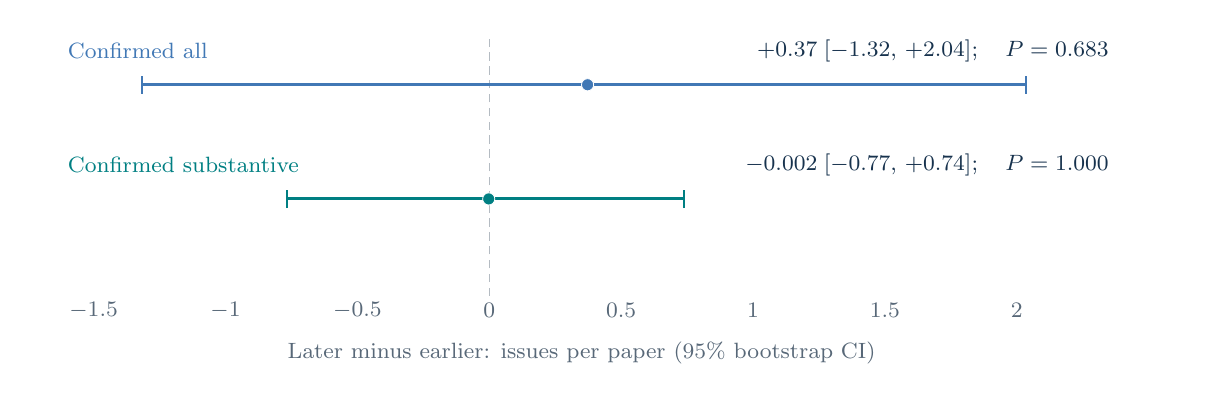
\begin{tikzpicture}[x=3.35cm,y=1.45cm,
  every node/.style={font=\fontsize{8}{10}\selectfont,inner sep=0pt}]
\path[use as bounding box] (-1.75,-.52) rectangle (2.7,2.5);
\draw[Slate!45,densely dashed] (0,.15) -- (0,2.4);
\draw[Blue,line width=1.1pt] (-1.31578947368421,2) -- (2.03584210526315,2);
\draw[Blue,line width=.7pt] (-1.31578947368421,2-.08) -- (-1.31578947368421,2+.08)
  (2.03584210526315,2-.08) -- (2.03584210526315,2+.08);
\filldraw[fill=Blue,draw=white,line width=.3pt] (0.37263157894737,2) circle[radius=2.2pt];
\node[anchor=west,text=Blue] at (-1.6,2+.3) {Confirmed all};
\node[anchor=east,text=Navy] at (2.35,2+.3) {$ +0.37\;[-1.32,\,+2.04];\quad P=0.683 $};
\draw[Teal,line width=1.1pt] (-0.76847368421053,1) -- (0.73684210526316,1);
\draw[Teal,line width=.7pt] (-0.76847368421053,1-.08) -- (-0.76847368421053,1+.08)
  (0.73684210526316,1-.08) -- (0.73684210526316,1+.08);
\filldraw[fill=Teal,draw=white,line width=.3pt] (-0.00210526315789,1) circle[radius=2.2pt];
\node[anchor=west,text=Teal] at (-1.6,1+.3) {Confirmed substantive};
\node[anchor=east,text=Navy] at (2.35,1+.3) {$ -0.002\;[-0.77,\,+0.74];\quad P=1.000 $};
\foreach \tick in {-1.5,-1,-0.5,0,0.5,1,1.5,2}
  \node[text=Slate] at (\tick,.02) {$\pgfmathprintnumber[fixed,precision=1]{\tick}$};
\node[text=Slate] at (.35,-.35) {Later minus earlier: issues per paper (95\% bootstrap CI)};
\end{tikzpicture}\par
\raggedright
\textcolor{Teal}{\textbf{Both intervals span decreases and increases; neither establishes equivalence.}}
\src{Source: slides/data/period\_comparisons.csv. Exact two-sided paper-level permutation $P$; separate percentile bootstrap CI. Confirmed-all comparison added for this presentation; confirmed substantive reproduces the paper's strict endpoint.}
% BEGIN EMBEDDED SPEECH NOTE
% Final judgments: review_results_2_4_1_Rbulun_copy/*.xlsx.
\note{
核心结果：全部确认略增，实质性均值近乎相同
\par
从最终工作簿逐条汇总，早期两年的已确认统计问题是 34 加 22，共 56 个；后期是 43 加 40，共 83 个。分别除以 19 篇和 25 篇论文，均值为 2.95 和 3.32，后期减早期约增加 0.37 个。这些是最终标签对应的实际计数。
\par
这项差值的 95\% bootstrap 置信区间是负 1.32 到正 2.04，精确置换 P 值为 0.683。也就是说，点估计略高，但不确定性范围同时包含减少和增加。
\par
实质性子集在早期是 11 加 5，共 16 个；后期是 11 加 10，共 21 个。两期论文数不同，换算后都约为每篇 0.84；差值约为负 0.002。对应区间为负 0.77 到正 0.74，精确置换 P 值为 1。
\par
下面两条区间都跨过零，所以目前的数据没有建立明确的时期差异。同时，P 值很大，也不能证明两个时期完全相同，或者已经达到统计学上的等效。这里能直接说的是：在这个样本中，全部确认问题的平均数略高，而确认且实质的问题均值近乎相同。
\par
转场：那么，全部确认口径里这约 0.37 个问题的增加，具体来自哪一部分？
}
% END EMBEDDED SPEECH NOTE
\end{frame}

\begin{frame}[t]{Presentation issues account for the count difference}
\small
\begin{tabularx}{\linewidth}{@{}Yrrr@{}}
\toprule
Mean issues per paper & Earlier & Later & Later $-$ earlier\\\midrule
Confirmed presentation only & 2.105 & 2.480 & $+0.375$\\
Confirmed substantive & 0.842 & 0.840 & $-0.002$\\\midrule
\textbf{Confirmed all} & \textbf{2.947} & \textbf{3.320} & \textbf{$+0.373$}\\\bottomrule
\end{tabularx}
\medskip
\textbf{A different question: how many papers contain at least one issue?}\par\smallskip
\small
\begin{tabularx}{\linewidth}{@{}Yrrrr@{}}
\toprule
Outcome & Earlier & Later & Difference (95\% CI), pp & $P$\\\midrule
Confirmed all & 16/19 (84.2\%) & 22/25 (88.0\%) & $+3.8$ ($-16.2$, $24.8$) & 1.000\\
Confirmed substantive & 8/19 (42.1\%) & 12/25 (48.0\%) & $+5.9$ ($-24.4$, $35.2$) & 0.766\\\bottomrule
\end{tabularx}
\takeaway{Nearly equal substantive means can coexist with a higher fraction of affected papers.}
\src{Source: slides/data/period\_comparisons.csv. pp = percentage points. Overall, 38/44 papers have a confirmed statistical finding; 20/44 have a confirmed substantive one. Count decomposition is descriptive.}
% BEGIN EMBEDDED SPEECH NOTE
% Final judgments: review_results_2_4_1_Rbulun_copy/*.xlsx.
\note{
变化分解：呈现问题与受影响论文比例
\par
上半部分把全部确认问题拆成两类。确认的呈现问题从每篇 2.105 个增加到 2.480 个，差值约为正 0.375；确认且实质的问题从 0.842 变成 0.840，差值约为负 0.002。两部分相加，就是全部确认问题约正 0.373 的变化。因此，这个均值差在数值上来自呈现问题的增加，并不表示实质性问题也增加了。
\par
下半部分换了一个问题：不是问每篇平均有多少个，而是问有多少篇至少出现一个。全部确认口径下，这个比例从 16 篇占 19 篇，也就是 84.2\%，变成 22 篇占 25 篇，也就是 88.0\%；增加了 3.8 个百分点。
\par
确认且实质的口径下，比例从 42.1\% 变成 48.0\%，增加了 5.9 个百分点。但两项比例差的置信区间都很宽，P 值分别为 1 和 0.766，仍然没有建立明确的时期差异。
\par
每篇平均问题数和至少有一个问题的论文比例，并不需要同步变化。一组问题可以分布在较少论文中，也可以分散在更多论文中。因此，实质性均值近乎相同，同时受影响论文比例略高，在数学上并不矛盾。
\par
转场：最后还要解释一个口径差异：为什么论文的主要分析看起来是下降，而这里的确认且实质均值几乎不变。
}
% END EMBEDDED SPEECH NOTE
\end{frame}

\begin{frame}[t]{The apparent decline comes from probable issues}
\begin{columns}[T,onlytextwidth]
\column{.48\textwidth}
\begin{block}{Earlier period: 2018--2019}
\centering\large
16 confirmed + 4 probable = \textbf{20}\par
\small substantive issues in 19 papers\par\medskip
Mean rises from \textbf{0.84} to \textbf{1.05}.
\end{block}
\column{.48\textwidth}
\begin{block}{Later period: 2024--2025}
\centering\large
21 confirmed + 0 probable = \textbf{21}\par
\small substantive issues in 25 papers\par\medskip
Mean remains \textbf{0.84}.
\end{block}
\end{columns}
\medskip
\small
\begin{tabularx}{\linewidth}{@{}Yrrr@{}}
\toprule
Substantive statistical endpoint & Mean difference & 95\% CI & $P$\\\midrule
Confirmed only & $-0.002$ & $-0.77$ to $0.74$ & 1.000\\
Confirmed + probable (paper principal) & $-0.21$ & $-1.02$ to $0.56$ & 0.654\\\bottomrule
\end{tabularx}
\takeaway{All four probable substantive findings are earlier: the apparent decline depends on including them.}
\smalltext
Other paper results: 1 earlier versus 3 later eligible substantive report-internal issues ($P=0.622$); combining them with the principal endpoint gives means 1.11 versus 0.96 ($P=0.754$).
\src{Source: manuscript Results and analysis/period\_comparisons.csv. Principal endpoint: 41 findings across 22/44 papers; confirmed substantive: 37 findings across 20/44 papers.}
% BEGIN EMBEDDED SPEECH NOTE
% Final judgments: review_results_2_4_1_Rbulun_copy/*.xlsx.
\note{
敏感性分析：纳入 probable 后为何出现下降
\par
关键就在这一页的四个 probable，也就是很可能存在、但尚未确认的实质性问题。它们全部来自早期组。
\par
如果只纳入确认且实质的问题，早期是 16 个，后期是 21 个，两期均值都约为 0.84。如果采用论文的主要结局，把很可能存在的实质性问题也算进去，早期就变成 16 加 4，合计 20 个，平均每篇 1.05 个；后期没有新增的 probable，所以仍然是 21 个，平均每篇 0.84 个。
\par
这样，后期减早期的差值就从接近零，变成负 0.21。论文主要结果中这个表面上的下降，正是由纳入早期这四个 probable 条目产生的。它的 95\% 置信区间是负 1.02 到正 0.56，P 值是 0.654，仍然不足以建立时期差异。
\par
这说明结论对证据确定程度的纳入标准有一定敏感性，两种口径都应透明报告。补充分析中，符合条件的实质性报告内部不一致是早期 1 个、后期 3 个；把它们和主要结局合并，均值为 1.11 对 0.96，P 值为 0.754，也没有改变整体解释。
\par
转场：除了统计结果，我们也按各自的审查规则比较另外三个领域。
}
% END EMBEDDED SPEECH NOTE
\end{frame}

\begin{frame}[t]{Extend the comparison to the other three review domains}
\small
% Embedded: tables/other_domains_broad.tex
\begin{tabularx}{\linewidth}{@{}Yrrrr@{}}
\toprule
Domain / eligible state & Before ($n=19$) & After ($n=25$) & $\Delta$ (95\% CI) & $P$ \\
\midrule
Report-internal: established & 0.16 [3] & 0.32 [8] & $+0.16$ ($-0.09$, $0.40$) & 0.301 \\
Plan material: established & 0.63 [12] & 0.68 [17] & $+0.05$ ($-0.51$, $0.65$) & 0.893 \\
Protocol--report: retained & 5.37 [102] & 4.48 [112] & $-0.89$ ($-2.38$, $0.60$) & 0.256 \\
\bottomrule
\end{tabularx}

\smallskip\par
\smalltext Mean findings per paper [total findings]; $\Delta$ = after minus before. Before: 2018--2019; after: 2024--2025.
\medskip
\begin{columns}[T,onlytextwidth]
\column{.48\textwidth}
\textbf{What ``all'' means in each domain}\par\medskip
\smalltext
\textbf{Report / plan:} retained and \code{substantive_inconsistency} or \code{minor_presentation}; indeterminate is excluded.\par\medskip
Report retained totals: 4 / 8; established: 3 / 8. Plan retained totals: 12 / 20; established: 12 / 17.
\column{.48\textwidth}
\textbf{Protocol--report remains descriptive}\par\medskip
\smalltext
All 102 / 112 retained differences are included here, regardless of optional interpretation. Interpretation is blank for 2 / 3 candidates.\par\medskip
Final human domains are used; original plan-related codes are allowed in this new extension.
\end{columns}
\takeaway{These are domain-specific outcomes; protocol differences are not confirmed errors.}
\src{Source: analysis/domain\_comparisons/. Exact two-sided paper permutation tests; separate 20,000-resample bootstrap CIs. Original statistical/report-only endpoints are unchanged. All comparisons are exploratory and do not estimate a pandemic effect.}
% BEGIN EMBEDDED SPEECH NOTE
% Final judgments: review_results_2_4_1_Rbulun_copy/*.xlsx.
\note{
其他三个领域：宽口径的前后比较
\par
其他三个领域也按最终工作簿 E 列的领域标签重新汇总。报告内部和计划材料的宽口径，要求 K 列是实质性不一致或轻微呈现不一致；保留但无法判断的条目不计入已建立问题。方案与报告领域的宽口径则统计全部保留差异，不能直接称为错误或违反方案。
\par
报告内部已建立的问题从 3 条到 8 条，每篇均值从 0.16 到 0.32，差值约正 0.16，P 值 0.301。计划材料从 12 条到 17 条，每篇从 0.63 到 0.68，差值约正 0.05，P 值 0.893。方案与报告保留差异从 102 条到 112 条，但按论文数换算，均值从 5.37 降到 4.48，差值约负 0.89，P 值 0.256。
\par
保留数与已建立数要分清：报告内部两期保留 4 条和 8 条，其中已建立 3 条和 8 条；计划材料保留 12 条和 20 条，其中已建立 12 条和 17 条。方案与报告保留差异中，解释字段有 2 条和 3 条为空；宽口径仍包括它们。三个均值差区间均跨过零。
\par
这些新增结果按最终领域标签定义，也纳入原始计划相关关系，因此不同于论文原来只分析报告材料的口径。它们是事后描述性扩展；与统计结果一起看时，必须保留各领域不同的计数含义。
\par
转场：下一页进一步只看各领域的实质性状态。
}
% END EMBEDDED SPEECH NOTE
\end{frame}

\begin{frame}[t]{Substantive findings are sparse outside the statistical domain}
\small
% Embedded: tables/other_domains_substantive.tex
\begin{tabularx}{\linewidth}{@{}Yrrrr@{}}
\toprule
Domain / eligible state & Before ($n=19$) & After ($n=25$) & $\Delta$ (95\% CI) & $P$ \\
\midrule
Report-internal: substantive & 0.05 [1] & 0.16 [4] & $+0.11$ ($-0.07$, $0.28$) & 0.370 \\
Plan material: substantive & 0.00 [0] & 0.16 [4] & $+0.16$ ($0.00$, $0.44$) & 0.498 \\
Protocol--report: substantive difference & 4.37 [83] & 3.84 [96] & $-0.53$ ($-1.85$, $0.74$) & 0.446 \\
\bottomrule
\end{tabularx}

\smallskip\par
\smalltext Mean findings per paper [total findings]; before = 2018--2019, after = 2024--2025. CI units: findings per paper.
\medskip
\begin{columns}[T,onlytextwidth]
\column{.48\textwidth}
\textbf{Papers with at least one substantive finding}\par\medskip
\smalltext
Report-internal: 1/19 $\rightarrow$ 4/25.\par
Plan material: 0/19 $\rightarrow$ 2/25.\par
Protocol--report: 18/19 $\rightarrow$ 24/25.\par\medskip
Four substantive plan findings are concentrated in \textbf{two later papers}; the earlier sample has zero.
\column{.48\textwidth}
\textbf{Reconcile with the paper's original endpoint}\par\medskip
\smalltext
Final-domain report-internal total: \textbf{5}. Original report-only eligible total: \textbf{4}.\par\medskip
\code{2024::jama.2024.11057::C003} was edited into the report-internal domain but retains original \code{P_R}; it enters this extension, not the original secondary endpoint.
\end{columns}
\takeaway{No clear period difference emerges; sparse counts and wide intervals limit interpretation.}
\src{Source: analysis/domain\_comparisons/. Substantive inconsistency for report/plan; substantive\_difference for protocol--report. A zero earlier sample produces a boundary bootstrap interval for plan findings; it does not establish absence in the underlying population.}
% BEGIN EMBEDDED SPEECH NOTE
% Final judgments: review_results_2_4_1_Rbulun_copy/*.xlsx.
\note{
其他三个领域：实质性结果与稀疏性
\par
报告内部实质性问题从 1 条到 4 条，每篇均值从 0.05 到 0.16，P 值 0.370。计划材料实质性问题从 0 条到 4 条，每篇从零到 0.16，P 值 0.498；这四条集中在后期两篇论文。方案与报告的实质性差异从 83 条到 96 条，但每篇均值从 4.37 降到 3.84，P 值 0.446。
\par
计划材料的早期观察值全为零，分层 bootstrap 无法从这些零里产生早期的非零值，所以区间下限为零。这并不证明真实发生率为零，也不能据此声称已经建立增长。样本稀疏时要同时看原始分布、重抽样局限和置换结果。
\par
原报告材料口径中，实质性报告内部问题是早期 1 条、后期 3 条；按最终领域标签汇总则是 1 条和 4 条。多出的条目是 2024 年 jama.2024.11057 的 C003：最终工作簿将其归为报告内部不一致且具有实质性，来源对照表记录的原始关系是 P\_R。因此它进入最终领域比较，但不进入原报告材料口径。
\par
方案与报告中的 substantive\_difference 仍是实质性差异的描述，不代表已经确认不当偏离。最终解释仍需要对应的计划版本、时间和理由。
\par
转场：最后回到统计问题，看看总均值之下的机制组成有没有不同。
}
% END EMBEDDED SPEECH NOTE
\end{frame}

\begin{frame}[t]{Which statistical mechanisms differ between publication cohorts?}
\small
% Embedded: tables/notes_category_period.tex
\begin{tabularx}{\linewidth}{@{}Yrrrr@{}}
\toprule
Statistical mechanism & Before: All & After: All & Before: Sub. & After: Sub. \\
\midrule
Counts / denominators & 13 / 0.68 & 26 / 1.04 & 1 / 0.05 & 3 / 0.12 \\
Effect estimates / estimands & 4 / 0.21 & 10 / 0.40 & 3 / 0.16 & 5 / 0.20 \\
Intervals / distribution summaries & 14 / 0.74 & 10 / 0.40 & 4 / 0.21 & 3 / 0.12 \\
P values / inference & 8 / 0.42 & 7 / 0.28 & 3 / 0.16 & 1 / 0.04 \\
Contrast sign / direction & 7 / 0.37 & 8 / 0.32 & 2 / 0.11 & 3 / 0.12 \\
Attribution / swaps / duplication & 7 / 0.37 & 5 / 0.20 & 3 / 0.16 & 3 / 0.12 \\
Analysis / measure definitions & 3 / 0.16 & 17 / 0.68 & 0 / 0.00 & 3 / 0.12 \\
\midrule
\textbf{Total} & \textbf{56 / 2.95} & \textbf{83 / 3.32} & \textbf{16 / 0.84} & \textbf{21 / 0.84} \\
\bottomrule
\end{tabularx}

\smallskip\par
\smalltext Each cell shows count / mean per paper. Before: 19 papers; after: 25 papers. All = confirmed; Sub. = confirmed substantive.
\medskip
% Embedded: tables/notes_period_takeaway.tex
\smalltext
\textbf{Composition changes beneath the similar substantive mean:} analysis/measure-definition candidates rise from 0.16 to 0.68 per paper; interval candidates fall from 0.74 to 0.40.\par\medskip
\textcolor{Teal}{\textbf{Mechanisms are post hoc descriptive categories, not evidence that pandemic exposure caused a change.}}

\src{Source: reconciled candidate-level Notes coding; all 44 papers retained in the denominators. Primary categories are mutually exclusive. These post hoc mechanism comparisons are descriptive; classification uncertainty and shared-model blind spots are not included in the original statistical intervals.}
% BEGIN EMBEDDED SPEECH NOTE
% Final judgments: review_results_2_4_1_Rbulun_copy/*.xlsx.
\note{
统计机制的前后分布：总量相似不等于组成相同
\par
这一页是补充机制分类的时期分布，不是直接从最终工作簿读取的新增字段。候选的纳入、年份和实质性采用最终结果；主要机制来自先前归档的 Notes 分类。每格先报候选数，再报每篇均值，早期分母为 19，后期为 25。
\par
全部确认中，人数与分母从 13 条到 26 条，每篇从 0.68 到 1.04；分析或测量定义从 3 条到 17 条，每篇从 0.16 到 0.68。区间与分布摘要则从 14 条到 10 条，每篇从 0.74 降到 0.40。说明两个时期的机制组成不同，即使总均值变化不大，也可能有方向相反的分项变化。
\par
实质性部分同样有抵消：分析定义从零到 3 条，效应量从 3 条到 5 条，而区间从 4 条到 3 条，推断从 3 条到 1 条。合计仍是早期 16 条、后期 21 条，换算后都约为每篇 0.84。
\par
这些机制是事后分类，部分记录还有分类歧义；本页没有另做类别层面的显著性检验。可以描述归档分类中的组成变化，但不能称为最终审查工作簿已经独立验证的机制差异，更不能归因于疫情。只有 139、37 及其按年份和论文分组的审查结果直接以最终标签为准。
\par
转场：最后用四点收束这次汇报。
}
% END EMBEDDED SPEECH NOTE
\end{frame}

\begin{frame}[t]{Keep evidence, mechanism and period interpretation distinct}
\begin{tabularx}{\linewidth}{@{}p{.55cm}Y@{}}
\textcolor{Teal}{\Large\textbf{1}} & \textbf{Study design:} compare 44 selected trial packages across the 2018--2019 and 2024--2025 publication cohorts, using final human-reviewed workbook decisions.\\[2mm]
\textcolor{Blue}{\Large\textbf{2}} & \textbf{Statistical findings:} confirmed all rises from 2.95 to 3.32 per paper; confirmed substantive remains about 0.84. Adding four earlier probable cases produces the paper's apparent decline.\\[2mm]
\textcolor{Navy}{\Large\textbf{3}} & \textbf{Broader comparison:} the other three domains show no clear period differences. Protocol--report differences remain descriptive; they are not pooled with confirmed statistical errors.\\[2mm]
\textcolor{Teal}{\Large\textbf{4}} & \textbf{Notes-based recategorization:} preserve all 440 raw notes; connect 139 confirmed cases to final human labels; classify mechanisms separately from the 37 substantive judgments.
\end{tabularx}
\medskip
\smalltext
Availability sampling, shared-model review histories and unmeasured missed findings limit generalization. Before/after are publication-cohort labels, not a causal estimate of pandemic effects. New mechanism coding needs human assessment before use as a validated taxonomy.
\src{Sources: raw reviewer Notes, final copied workbooks and reproducible extension analyses. User confirmed later human review of copied workbooks; raw Notes remain AI-authored. The prior 15-slide version is archived.}
% BEGIN EMBEDDED SPEECH NOTE
% Final judgments: review_results_2_4_1_Rbulun_copy/*.xlsx.
\note{
结束：把证据、判断、机制与时期比较连接起来
\par
第一，全部确认的统计问题均值从每篇 2.95 到 3.32，约增加 0.37，数值变化来自呈现问题。确认且实质的均值则约为 0.84 对 0.84。区间仍较宽，不能说已证明没有变化或达到等效。
\par
第二，另外三个领域已经分别补充前后比较，但都没有建立明确的时期差异。报告不一致、计划材料问题，以及方案报告差异，各自的定义必须保留，尤其不能把所有方案差异都称为错误。
\par
第三，本次以四份 completed 工作簿为结果依据：440 条候选中保留 413 条、排除 27 条，全部完成。codebook 把处置、确定性和实质性分开，只有先说明筛选条件，139、37 和 41 这几个数量才可解释。
\par
第四，最终工作簿中保留条目的 Notes 为空。七类机制和两个详细例子来自另外归档的原始说明，是补充分析；本次核对了它们与最终候选及实质性标签的一致性。这些结果属于探索性样本分析，不能估计所有真实问题的漏检率，也不能说明疫情造成了变化。谢谢大家。
}
% END EMBEDDED SPEECH NOTE
\end{frame}

\end{document}
